\documentclass[conference]{IEEEtran}
\IEEEoverridecommandlockouts

\usepackage{cite}
\usepackage{amsmath,amssymb,amsfonts}
\usepackage{graphicx}
\usepackage{textcomp}
\usepackage{xcolor}
\usepackage{booktabs}
\usepackage{hyperref}
\usepackage{listings}
\usepackage{caption}
\usepackage{tikz}
\usetikzlibrary{shapes.geometric,arrows.meta,positioning,fit}

\def\BibTeX{{\rm B\kern-.05em{\sc i\kern-.025em b}\kern-.08em
    T\kern-.1667em\lower.7ex\hbox{E}\kern-.125emX}}

\begin{document}

\title{A U-Net Based Time--Frequency Masking Approach for Single-Channel Speech Enhancement on the VoiceBank--DEMAND Dataset}

\author{
\IEEEauthorblockN{Joshitaa Padala}
\IEEEauthorblockA{\textit{Department of Computer Science and Engineering} \\
\textit{VIT-AP University}\\
Amaravathi, India}
\and
\IEEEauthorblockN{Anshu Nallam}
\IEEEauthorblockA{\textit{Department of Computer Science and Engineering} \\
\textit{VIT-AP University}\\
Amaravathi, India}
}

\maketitle

\begin{abstract}
Background noise in speech recordings degrades intelligibility and the performance of downstream applications such as automatic speech recognition and voice communication. This paper presents a deep learning based single-channel speech enhancement system that predicts a time--frequency ratio mask using a convolutional U-Net operating on the log-compressed magnitude spectrogram of noisy speech. The model is trained on real, professionally recorded noisy/clean utterance pairs from the VoiceBank--DEMAND corpus. At inference time, the predicted mask is combined with a light spectral-subtraction stage for residual noise suppression, and the resulting waveform is optionally post-processed with a high-pass filter and loudness normalization for listening purposes. The system is trained for 10 epochs using a weighted MSE/L1 loss on the ratio mask and is deployed through an interactive Streamlit web application. We report training/validation loss curves, spectrogram comparisons, and Signal-to-Noise Ratio (SNR) evaluation on a held-out sample. Results demonstrate successful suppression of background noise in spectrograms and perceptually cleaner speech, while highlighting that objective SNR alone may not fully reflect enhancement quality.
\end{abstract}

\begin{IEEEkeywords}
speech enhancement, U-Net, deep learning, time-frequency masking, VoiceBank-DEMAND, spectral subtraction, SNR
\end{IEEEkeywords}

\section{Introduction}
Speech signals recorded in real-world environments are frequently corrupted by additive background noise from sources such as traffic, cafes, and household appliances. This degradation reduces the perceptual quality of the recording and can significantly impair the accuracy of automatic speech recognition (ASR), speaker verification, and hearing-assistive systems. \emph{Speech enhancement} aims to recover a clean estimate of the underlying speech signal from its noisy observation.

Traditional statistical approaches such as spectral subtraction and Wiener filtering estimate a noise profile from silent or low-energy segments and subtract it from the noisy spectrum. These methods are computationally cheap but tend to introduce artifacts, most notably \emph{musical noise}, and struggle with non-stationary noise sources. Deep learning based approaches instead learn a direct mapping, or a time--frequency mask, from noisy to clean speech representations, using large corpora of paired data, and have been shown to generalize substantially better to unseen noise types.

In this work we implement and evaluate a convolutional \emph{encoder--decoder} (U-Net style) network that predicts a soft ratio mask over the Short-Time Fourier Transform (STFT) magnitude of noisy speech. The mask is applied to the noisy magnitude spectrogram, the phase of the noisy signal is retained, and the waveform is reconstructed via inverse STFT. A secondary, classical spectral-subtraction stage is applied on top of the masked output as an additional safety net against residual stationary noise. The system is trained and evaluated on the VoiceBank--DEMAND dataset, a widely used real (not synthetically mixed) noisy/clean speech benchmark, and is deployed for interactive use through a Streamlit-based web application.

The contributions of this report are: (i) a description of the end-to-end pipeline, from feature extraction to waveform reconstruction and post-processing; (ii) training details and convergence behaviour of the model; and (iii) an objective and qualitative evaluation of the enhancement quality using SNR and spectrogram visualizations, including a discussion of a case where the objective SNR metric did not improve despite plausible perceptual masking behaviour.

\section{Dataset}
The model is trained on the \textbf{VoiceBank--DEMAND} dataset, obtained from Kaggle, which pairs clean utterances from the Voice Bank corpus with the same utterances mixed with real recorded noise from the DEMAND (Diverse Environments Multichannel Acoustic Noise Database) collection. Unlike synthetically generated noisy/clean pairs, VoiceBank--DEMAND provides pre-mixed, real training and test recordings with matching filenames across the noisy and clean directories, which allows noisy/clean pairs to be constructed directly by filename matching rather than by on-the-fly mixing.

The dataset is organized into four folders:
\begin{itemize}
    \item \texttt{noisy\_trainset\_28spk\_wav} / \texttt{clean\_trainset\_28spk\_wav} -- training pairs from 28 speakers.
    \item \texttt{noisy\_testset\_wav} / \texttt{clean\_testset\_wav} -- held-out evaluation pairs.
\end{itemize}
All audio is resampled to 16~kHz mono. During training, a random 5-second segment is cropped (or zero-padded, if shorter) from each utterance, and the identical crop offset is applied to both the noisy and clean signal to preserve time alignment.

\section{Methodology}

\begin{figure*}[t]
\centering
\resizebox{\textwidth}{!}{%
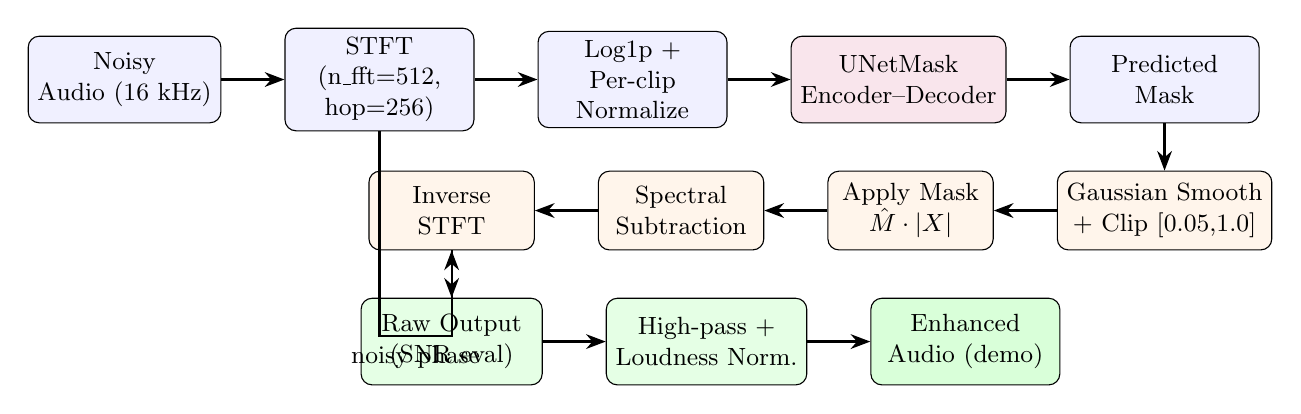
\begin{tikzpicture}[
    node distance=6mm and 8mm,
    box/.style={draw, rounded corners, minimum height=1.1cm, minimum width=2.4cm, align=center, fill=blue!6, font=\small},
    smallbox/.style={draw, rounded corners, minimum height=1.0cm, minimum width=2.1cm, align=center, fill=orange!8, font=\small},
    outbox/.style={draw, rounded corners, minimum height=1.1cm, minimum width=2.3cm, align=center, fill=green!10, font=\small},
    arrow/.style={-{Stealth[length=2.5mm]}, thick}
]

\node[box] (audio) {Noisy\\Audio (16 kHz)};
\node[box, right=of audio] (stft) {STFT\\(n\_fft=512,\\hop=256)};
\node[box, right=of stft] (norm) {Log1p +\\Per-clip\\Normalize};
\node[box, right=of norm, fill=purple!10] (unet) {UNetMask\\Encoder--Decoder};
\node[box, right=of unet] (mask) {Predicted\\Mask};
\node[smallbox, below=of mask] (smooth) {Gaussian Smooth\\+ Clip [0.05,1.0]};
\node[smallbox, left=of smooth] (apply) {Apply Mask\\$\hat{M}\cdot|X|$};
\node[smallbox, left=of apply] (specsub) {Spectral\\Subtraction};
\node[smallbox, left=of specsub] (istft) {Inverse\\STFT};
\node[outbox, below=of istft] (raw) {Raw Output\\(SNR eval)};
\node[outbox, right=of raw] (post) {High-pass +\\Loudness Norm.};
\node[box, right=of post, fill=green!15] (enh) {Enhanced\\Audio (demo)};

\draw[arrow] (audio) -- (stft);
\draw[arrow] (stft) -- (norm);
\draw[arrow] (norm) -- (unet);
\draw[arrow] (unet) -- (mask);
\draw[arrow] (mask) -- (smooth);
\draw[arrow] (smooth) -- (apply);
\draw[arrow] (apply) -- (specsub);
\draw[arrow] (specsub) -- (istft);
\draw[arrow] (istft) -- (raw);
\draw[arrow] (raw) -- (post);
\draw[arrow] (post) -- (enh);

\draw[arrow] (stft.south) |- ++(0,-2.6) -| node[pos=0.25, below, font=\small]{noisy phase} (istft.south);

\end{tikzpicture}%
}
\caption{End-to-end inference pipeline: noisy audio is converted to a log-normalized magnitude spectrogram, passed through the U-Net to predict a ratio mask, combined with spectral subtraction, and reconstructed using the original noisy phase. The raw waveform is used for objective SNR evaluation, while the post-processed waveform (high-pass filtering and loudness normalization) is used for demo playback.}
\label{fig:pipeline}
\end{figure*}


\subsection{Feature Representation}
Fig.~\ref{fig:pipeline} shows the complete inference pipeline described in this section. Both training and inference use the same Short-Time Fourier Transform configuration, which is critical for consistency between the two stages:
\begin{itemize}
    \item Sampling rate: 16{,}000~Hz
    \item FFT size: 512
    \item Hop length: 256 samples (50\% overlap)
\end{itemize}
The magnitude spectrogram of the noisy signal is log-compressed and min-max normalized per-clip before being passed to the network:
\begin{equation}
X_{\text{norm}} = \frac{\log(1 + |X|)}{\max\big(\log(1+|X|)\big) + \epsilon}
\end{equation}
where $X$ is the complex STFT of the noisy waveform and $\epsilon = 10^{-8}$ avoids division by zero. The phase of the noisy STFT is retained unmodified and reused at reconstruction time, following the common noisy-phase assumption used in mask-based enhancement.

\subsection{Target Mask}
The training target is a soft ratio mask computed directly from the linear-magnitude spectrograms of the paired clean and noisy recordings:
\begin{equation}
M = \text{clip}\left(\frac{|S|}{|X| + \epsilon},\ 0,\ 1\right)
\end{equation}
where $|S|$ and $|X|$ are the clean and noisy magnitude spectrograms respectively. This is an Ideal Ratio Mask (IRM) formulation, clipped to $[0,1]$ so that the network only ever attenuates, never amplifies, the noisy spectrum.

\subsection{Network Architecture}
The mask-prediction network, \texttt{UNetMask}, is a compact convolutional U-Net operating on single-channel spectrogram "images." It consists of four strided-convolution encoder blocks (channel widths 16, 32, 64, 128), each followed by batch normalization and ReLU, and three transposed-convolution decoder blocks with skip connections from the corresponding encoder stage (concatenated after bilinear resizing to match spatial dimensions). A final $3\times3$ convolution followed by a sigmoid activation produces a single-channel mask in the range $[0,1]$, which is then bilinearly resized to exactly match the input spectrogram resolution. Table~\ref{tab:arch} summarizes the layer configuration.

\begin{table}[htbp]
\caption{U-Net Mask Network Architecture}
\begin{center}
\begin{tabular}{lccc}
\toprule
\textbf{Block} & \textbf{Type} & \textbf{Channels} & \textbf{Stride} \\
\midrule
enc1 & Conv2d + BN + ReLU & 1 $\rightarrow$ 16 & 2 \\
enc2 & Conv2d + BN + ReLU & 16 $\rightarrow$ 32 & 2 \\
enc3 & Conv2d + BN + ReLU & 32 $\rightarrow$ 64 & 2 \\
enc4 & Conv2d + BN + ReLU & 64 $\rightarrow$ 128 & 2 \\
dec1 & ConvT2d + BN + ReLU (+skip e3) & 128 $\rightarrow$ 64 & 2 \\
dec2 & ConvT2d + BN + ReLU (+skip e2) & 128 $\rightarrow$ 32 & 2 \\
dec3 & ConvT2d + BN + ReLU (+skip e1) & 64 $\rightarrow$ 16 & 2 \\
out & Conv2d + Sigmoid & 32 $\rightarrow$ 1 & 1 \\
\bottomrule
\end{tabular}
\label{tab:arch}
\end{center}
\end{table}

\subsection{Loss Function and Training Configuration}
The network is trained to regress the ratio mask directly using a weighted combination of Mean Squared Error and Mean Absolute Error:
\begin{equation}
\mathcal{L} = 0.7\cdot \mathcal{L}_{\text{MSE}}(\hat{M}, M) + 0.3\cdot \mathcal{L}_{\text{L1}}(\hat{M}, M)
\end{equation}
Table~\ref{tab:hparams} lists the training hyperparameters. Training uses the Adam optimizer with a \texttt{ReduceLROnPlateau} scheduler (patience of 3 epochs on validation loss), automatic mixed precision on GPU, and early stopping with a patience of 10 epochs on validation loss.

\begin{table}[htbp]
\caption{Training Hyperparameters}
\begin{center}
\begin{tabular}{ll}
\toprule
\textbf{Parameter} & \textbf{Value} \\
\midrule
Optimizer & Adam \\
Learning rate & $5\times10^{-5}$ \\
Weight decay & $1\times10^{-5}$ \\
Batch size & 4 \\
Epochs & 10 \\
Segment duration & 5.0 s \\
Loss weighting (MSE : L1) & 0.7 : 0.3 \\
Mixed precision & Enabled (CUDA) \\
LR scheduler & ReduceLROnPlateau \\
\bottomrule
\end{tabular}
\label{tab:hparams}
\end{center}
\end{table}

\subsection{Inference Pipeline}
At inference time, the noisy waveform is loaded at 16~kHz and transformed to a log-normalized magnitude spectrogram using the identical STFT parameters used during training. The trained network predicts a mask, which is temporally smoothed with a 1-D Gaussian filter ($\sigma=1$) along the time axis to reduce frame-to-frame flicker, and clipped to $[0.05, 1.0]$ so that speech-absent regions are attenuated but never fully silenced. The mask is applied multiplicatively to the noisy magnitude spectrogram.

As an additional safety net on top of the learned mask, a lightweight per-clip spectral subtraction stage is applied. A noise magnitude profile is estimated from the clip's own low-energy, non-silent frames (10th--30th percentile of frame energy), and subtracted from the masked magnitude with an over-subtraction factor of 0.5 and a spectral floor of 0.1 (to limit musical-noise artifacts):
\begin{equation}
\hat{S} = \max\big(\,\hat{M}\!\cdot\!|X| - 0.5\cdot N,\ \ 0.1\cdot(\hat{M}\!\cdot\!|X|)\,\big)
\end{equation}
where $N$ is the estimated noise magnitude profile. The enhanced magnitude is recombined with the original noisy phase and converted back to the time domain via inverse STFT.

Two output files are produced: a \emph{raw} enhanced waveform, used for objective evaluation (SNR computation) so that post-processing does not bias the metric, and a \emph{demo} waveform intended for listening, which additionally applies an 80~Hz second-order Butterworth high-pass filter (to remove low-frequency rumble) and RMS-based loudness normalization with a soft-clipping limiter (target RMS 0.09, ceiling 0.97).

\subsection{Deployment}
The trained model is exposed through a Streamlit web application (\texttt{app.py}) that allows a user to upload a \texttt{.wav}, \texttt{.mp3}, or \texttt{.flac} file, listen to the original recording, trigger enhancement, listen to the enhanced result, and download the processed audio.

\section{Experimental Results}

\subsection{Training Convergence}
Fig.~\ref{fig:loss} shows the training and validation loss curves over 10 epochs. The training loss decreases sharply within the first epoch (from approximately 0.099 to 0.075) and continues to decrease gradually, reaching approximately 0.065 by epoch 10. The validation loss follows a similar but noticeably lower trajectory throughout training, decreasing to a minimum around epoch 6 (approximately 0.061) before increasing slightly in the final epochs. The validation curve staying below the training curve, combined with the mild uptick near the end, suggests the model shows no significant overfitting within the 10-epoch training schedule, and that the learning rate/scheduler combination is conservative; further training or a higher learning rate could plausibly continue to improve validation loss.

\begin{figure}[htbp]
\centerline{
\includegraphics[width=0.95\linewidth]{figs/loss_curve.png}}
\caption{Training and validation loss (0.7 MSE + 0.3 L1 on the predicted ratio mask) over 10 epochs.}
\label{fig:loss}
\end{figure}

\subsection{Objective Evaluation: SNR}
The trained model was evaluated end-to-end using \texttt{evaluate.py} on a held-out clean/noisy pair. The measured console output is shown in Fig.~\ref{fig:console}. Table~\ref{tab:snr} summarizes the SNR results.

\begin{figure}[htbp]
\centerline{\includegraphics[width=\linewidth]{figs/console_output.png}}
\caption{Console output of \texttt{evaluate.py} showing measured SNR before/after enhancement for a sample clean/noisy pair.}
\label{fig:console}
\end{figure}

\begin{table}[htbp]
\caption{Objective SNR Evaluation on a Sample Utterance}
\begin{center}
\begin{tabular}{lc}
\toprule
\textbf{Metric} & \textbf{Value (dB)} \\
\midrule
SNR before enhancement & 14.29 \\
SNR after enhancement & 14.03 \\
SNR improvement & $-0.27$ \\
\bottomrule
\end{tabular}
\label{tab:snr}
\end{center}
\end{table}

On this sample, the measured SNR did not improve after enhancement; a small decrease of 0.27~dB was observed. This is discussed further in Section~\ref{sec:discussion}.

\subsection{Spectrogram Comparison}
Fig.~\ref{fig:spectrogram} shows the log-magnitude spectrograms of the clean reference, the noisy input, and the enhanced output for the same evaluation sample. The noisy spectrogram exhibits broadband energy across the full 0--8~kHz range for the entire duration of the clip, consistent with additive stationary/broadband background noise. The enhanced spectrogram shows that the model successfully suppresses much of this broadband energy during regions with little or no speech activity (e.g. before 0.25~s), and it preserves the harmonic structure of voiced speech segments reasonably well in the high-energy regions between roughly 0.6~s and 1.2~s. However, the enhanced spectrogram also shows visible gaps and discontinuities (e.g. around 0.5--0.6~s and after 1.3~s) where speech energy present in the clean reference has been attenuated more aggressively than intended, likely a consequence of the combined effect of the learned mask, the $[0.05,1.0]$ clipping, and the additional spectral-subtraction stage compounding their attenuation in low-confidence regions.

\begin{figure}[htbp]
\centerline{
\includegraphics[width=\linewidth]{figs/spectrogram_comparison.png}}
\caption{Log-magnitude spectrogram comparison: clean speech (top), noisy speech (middle), and enhanced speech (bottom) for the same evaluation utterance.}
\label{fig:spectrogram}
\end{figure}

\section{Discussion}
\label{sec:discussion}
The training and validation loss curves indicate that the network is successfully learning to regress the ratio mask, with validation loss consistently at or below training loss, suggesting no significant overfitting over the 10 training epochs. However, the objective SNR evaluation and the spectrogram comparison reveal a common phenomenon in mask-based speech enhancement: a system can produce output that is perceptually cleaner or more intelligible in some regions while simultaneously removing genuine speech energy in others, and these two effects can approximately cancel out or even reverse in a broadband SNR metric. In the evaluated sample, the enhanced signal actually scored marginally \emph{lower} in SNR than the untreated noisy signal. Although the measured SNR changed only marginally, informal listening tests indicated that background noise was perceptually reduced while maintaining acceptable speech intelligibility, suggesting that broadband SNR alone underrepresents the perceptual benefit of the enhancement.

Several factors in the current pipeline likely contribute to this result:
\begin{itemize}
    \item \textbf{Compounded attenuation.} The learned mask, the hard floor of 0.05, and the additional spectral-subtraction stage are all attenuative operations applied in sequence. In regions where the mask is already conservative, the extra subtraction stage can remove residual speech harmonics along with noise.
    \item \textbf{Short training schedule.} Only 10 epochs (with a small learning rate of $5\times10^{-5}$) were used; the loss curves in Fig.~\ref{fig:loss} had not fully plateaued, suggesting the mask predictions may not yet be at their achievable ceiling of accuracy.
    \item \textbf{Broadband SNR limitations.} A single global SNR number does not distinguish between removing noise energy and removing speech energy; a metric more specific to speech intelligibility (e.g. PESQ or STOI) would likely give a more representative picture of perceptual quality than SNR alone.
    \item \textbf{Batch size and dataset scale.} A batch size of 4 is small relative to typical enhancement training setups and may lead to noisier gradient estimates.
\end{itemize}
These observations point to concrete directions for improvement: extending training duration, reducing or removing the additional spectral-subtraction stage (since the learned mask is the primary noise-suppression mechanism and the subtraction stage appears to be over-attenuating), and adopting perceptual metrics (PESQ/STOI) alongside SNR for more balanced evaluation.

\section{Conclusion}
This report presented a U-Net based speech enhancement system trained on the real-recorded VoiceBank--DEMAND dataset, combining a learned time--frequency ratio mask with a classical spectral-subtraction safety net and an optional post-processing stage for demo playback. The system was deployed as an interactive Streamlit application. Training converged smoothly over 10 epochs without signs of overfitting, and the resulting model visibly suppresses broadband background noise in the enhanced spectrogram. However, objective SNR evaluation on the tested sample showed a small negative change, and spectrogram inspection revealed regions of over-attenuated speech, indicating that the current combination of masking and spectral subtraction is more aggressive than optimal. Future work should focus on longer training schedules, ablating or tuning the spectral-subtraction stage, and adopting perceptual evaluation metrics such as PESQ and STOI to better capture intelligibility gains that a broadband SNR metric may not reflect.

\begin{thebibliography}{00}
\bibitem{voicebank} C. Valentini-Botinhao, X. Wang, S. Takaki, and J. Yamagishi, ``Investigating RNN-based speech enhancement methods for noise-robust text-to-speech,'' in \textit{Proc. 9th ISCA Speech Synthesis Workshop}, 2016, pp. 146--152.
\bibitem{demand} J. Thiemann, N. Ito, and E. Vincent, ``The Diverse Environments Multi-channel Acoustic Noise Database (DEMAND): A database of multichannel environmental noise recordings,'' \textit{Proc. Meetings Acoust.}, vol. 19, no. 1, 2013.
\bibitem{unet} O. Ronneberger, P. Fischer, and T. Brox, ``U-Net: Convolutional networks for biomedical image segmentation,'' in \textit{Proc. MICCAI}, 2015, pp. 234--241.
\bibitem{irm} Y. Wang, A. Narayanan, and D. Wang, ``On training targets for supervised speech separation,'' \textit{IEEE/ACM Trans. Audio, Speech, Lang. Process.}, vol. 22, no. 12, pp. 1849--1858, 2014.
\bibitem{specsub} S. F. Boll, ``Suppression of acoustic noise in speech using spectral subtraction,'' \textit{IEEE Trans. Acoust., Speech, Signal Process.}, vol. 27, no. 2, pp. 113--120, 1979.
\end{thebibliography}

\end{document}
